\documentclass{article}
\usepackage[utf8]{inputenc}
\usepackage[a4paper, total={6.5in, 9in}]{geometry}
\usepackage{fancyhdr}
\usepackage{amsmath, amsthm, amsfonts}
\usepackage[mathscr]{euscript}
\let\euscr\mathscr \let\mathscr\relax
\usepackage{xcolor, graphicx, subfig, float}

% \renewcommand{\headrulewidth}{0pt}
\setlength{\headsep}{4em}
\pagestyle{fancy}

% ASSIGNMENT INFORMATION
\newcommand{\class}{CS 671}
\newcommand{\hwnumber}{1}

\lhead{Braden Hoagland (bch29)}
\chead{{\class} - HW \hwnumber}
\rhead{\today}

\begin{document}

\section{Information Theory}
\begin{enumerate}
    \item
    For $n$ possible outcomes, the maximum entropy is $p_i = \frac{1}{n}$ for all $i$. To show this, we can optimize the Lagrangian \[\mathcal{L}(p, \lambda) = -\sum_i p_i \log(p_i) - \lambda \big(\sum_i p_i - 1\big)\]
    where the constraint forces $p$ to be a valid probability distribution. Setting $\frac{\partial \mathcal{L}}{\partial p_i}$ to 0 gives
    \begin{align*}
        \log_2 p_i + \frac{1}{\ln 2} + \lambda &= 0 \\
        p_i &= 2^{-((1/\ln 2) + \lambda)}
    \end{align*}
    This is clearly constant for all $i$, so the only possible value for $p_i$ is $p_i = \frac{1}{n}$. This is the uniform distribution.
    
    The maximum value of the entropy is then
    \begin{align*}
        \sum_{i=1}^n \frac{1}{n} \log_2 \frac{1}{n} &= n \cdot \frac{1}{n} \log_2 \frac{1}{n} \\
        &= \log_2 \frac{1}{n}
    \end{align*}
    
    \item
    The mutual information between $X$ and itself is just the entropy of $X$.
    \begin{align*}
        I(X,X) &= H(X) - H(X|X) \\
        &= H(X) - \sum_i H(X | X=x_i) p(x_i) \\
        &= H(X) - \sum_i 0 \cdot p(x_i) \\
        &= H(X)
    \end{align*}
    
    \item
    \begin{enumerate}
        \item
        Let $L(p,q) = \sum_i p_i \log_2 \frac{p_i}{q_i}$. We can start by showing that $L(p,q) \geq 0$. Since $L(p,q)$ more closely resembles $\log_2 x$ than $(x-a) \log_2 e$, it may be algebraically simpler to prove that $-L(p,q) \leq 0$, which implies $L(p,q) \geq 0$.
        
        \begin{align*}
            -L(p,q) &= -\sum_i p_i \log_2 \frac{p_i}{q_i} \\
            &= \sum_i p_i \log_2 \frac{q_i}{p_i} \\
            &\leq \sum_i p_i \left( \frac{q_i}{p_i} - 1 \right) \log_2 e \\
            &= \log_2 e \sum_i (q_i - p_i) \\
            &= \log_2 e \left[ \left( \sum_i p_i \right) - \left( \sum_i q_i \right) \right] \\
            &= \log_2 e (1-1) \\
            &= 0
        \end{align*}
        This gives the desired inequality.
        
        \item
        We can now show let $I(X,Y) = \sum_i \sum_j p(x_i,y_j) \log_2 \frac{p(x_i, y_j)}{p(x_i) p(y_j)}$.
        \begin{align*}
            I(X,Y) &= - \sum_i p(x_i) \log p(x_i) - \sum_j H(X | Y=y_j)p(y_j)
            \intertext{Partitioning the $p(x_i)$ on the left and expanding the conditional entropy term gives}
            &= - \sum_i \sum_j p(x_i, y_j) \log p(x_i) + \sum_j \sum_i p(x_i | y_j) \log p(x_i | y_j)p(y_j)
            \intertext{Rewriting the conditional probabilities and swapping the order of the last two summations gives}
            &= -\sum_i \sum_j p(x_i, y_j) \log p(x_i) + \sum_i \sum_j p(x_i, y_j) \log \frac{p(x_i, y_j)}{p(y_j)} \\
            &= \sum_i \sum_j p(x_i, y_j) \left[ \log \frac{p(x_i, y_j)}{p(y_j)} - \log p(x_i) \right] \\
            &= \sum_i \sum_j p(x_i, y_j) \log \frac{p(x_i, y_j)}{p(x_i) p(y_j)}
        \end{align*}
        This is the desired form.
    \end{enumerate}
    
	This sum can be expanded into two separate sums
	\[
		\sum_i \sum_j p(x_i, y_j) \log_2 \frac{p(x_i, y_j)}{p(y_j)} + \sum_i -\log_2 p(x_i) \sum_j p(x_i, y_j)
	\] 
	Since $\sum_{i} \sum_j p(x_i, y_j) = 1$ for categorically distributed $x_i$ and $y_j$ (which makes it a valid probability distribution), the double summation is in the form of the equation in part (a). Thus the first term is non-negative. Since $-\log_2 p(x_i)$ is non-negative for all probabilities $p(x_i)$, the second double summation is non-negative as well. Since both terms are non-negative, so is their sum. Thus $I(X,Y) \geq 0$.

\item
	To decide on which feature to split, we must find the entropy of the whole dataset and then find which feature reduces that entropy the most.

	The base entropy is $H(Y) = H([\frac{9}{14}, \frac{5}{14}])$. The entropies conditioned on each feature are
	\begin{align*}
		H(Y|\text{Outlook}) &= \frac{9}{14} H\Big(\Big[\frac{6}{9}, \frac{3}{9}\Big]\Big) + \frac{5}{14} H\Big(\Big[\frac{3}{5}, \frac{2}{5}\Big]\Big) \\
		H(Y|\text{Humidity}) &= \frac{7}{14} H\Big(\Big[\frac{6}{7}, \frac{1}{7}\Big]\Big) + \frac{7}{14} H\Big(\Big[\frac{3}{7}, \frac{4}{7}\Big]\Big) \\
		H(Y|\text{Windy}) &= \frac{8}{14} H\Big(\Big[\frac{6}{8}, \frac{2}{8}\Big]\Big) + \frac{6}{14} H\Big(\Big[\frac{3}{6}, \frac{3}{6}\Big]\Big)
	\end{align*}
	The information gain for each feature is then $H(Y) - H(Y|\text{feature})$, which computes to
	\begin{align*}
		\text{Gain}(Y, \text{Outlook}) &\approx 0.0032 \\
		\text{Gain}(Y, \text{Humidity}) &\approx 0.1518 \\
		\text{Gain}(Y, \text{Windy}) &\approx 0.0481
	\end{align*}
	Based on these values, we should split on the humidity feature, since it gives us the highest information gain.
\end{enumerate}

\section{Decision Trees}

\begin{enumerate}
	\item
		The following decision tree, with splits determined by the C4.5 algorithm, had a training error of $2/14 \approx 0.14$ and a test error of  $2/5 = 0.4$.
		\begin{figure}[H]
			\centering
			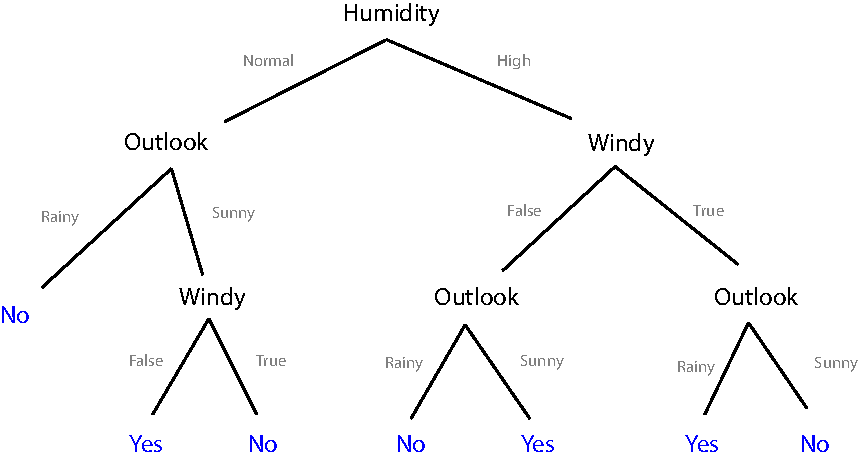
\includegraphics[scale=0.75]{img/tree.pdf}
		\end{figure}
	
	\item
		If we only split when the information gain is at least $0.04$, then the right side of the tree is never formed. This version of the tree has a training error of $3/14 \approx 0.214$ and a test error of $1/5 = 0.2$. The better test performance is most likely due to the tree not overfitting to the training set in instances of high entropy.

		In the case of high humidity, the other features did not provide enough information to warrant splitting. Because of the high entropy, further splitting provided little modeling improvement but still fit the tree more closely to the training set. By eliminating this source of overfitting, the model was able to more easily generalize.
		\begin{figure}[H]
			\centering
			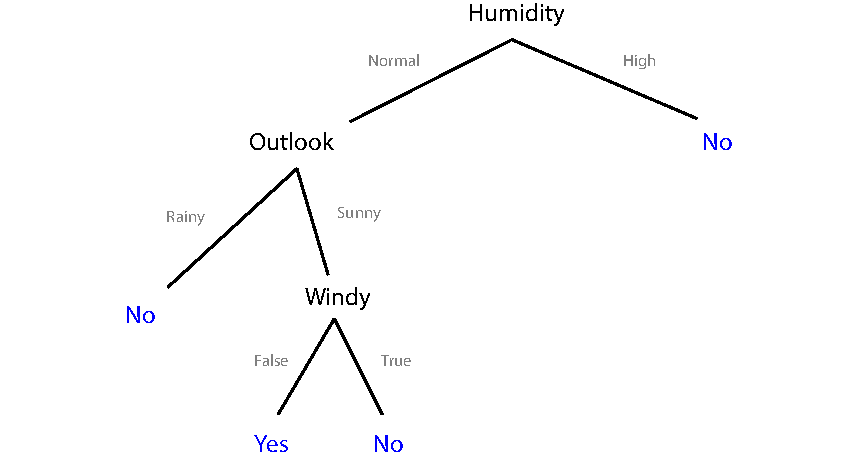
\includegraphics[scale=0.75]{img/pruned.pdf}
		\end{figure}
	
	\item 
		When constructing the tree using the Gini index for splitting, the same original tree as with C4.5 is created (training error is $2/14$, test error is $1/5$). The main difference comes during pruning, where we attempt to balance the number of leaves with the number of misclassified points. During the pruning, there are several points where we have a tie between the value of splitting and pruning. Depending on how these ties are settled, we could either end up with a tree identical to the pruned C4.5 tree, a tree that predicts ``Yes" for every point, or a tree that looks like the following.
		\begin{figure}[H]
			\centering
			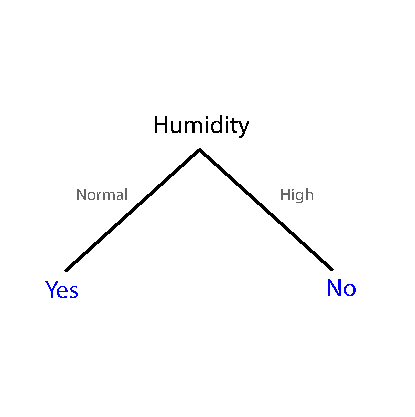
\includegraphics[scale=0.75]{img/cart-tree.pdf}
		\end{figure}

		In the case of this latter tree, the training error is $4/14 \approx 0.29$ and the test error is $1/5 = 0.2$. It has clearly traded increased training error for better generalization. As expected with CART, this tree is easier to interpret, using only one feature to make a decision.
\end{enumerate}


\section{Programming}

\begin{enumerate}
\item 
\begin{enumerate}
	\item
		The results of cross-validation for evlauation on the three methods is summarized below. The values given are the mean and standard deviation of the validation accuracy.
		\begin{center}
			\begin{tabular}{ |c|c|c| }
				\hline
				\multicolumn{3}{|c|}{Cross-Validation Accuracy} \\
				\hline
				& $\mu$ & $\sigma$ \\
				\hline
				Random Forest & 0.9604 & 0.0088 \\
				CART & 0.9231 & 0.0197 \\
				ID3 & 0.9341 & 0.0155 \\
				\hline
			\end{tabular}
		\end{center}
		After performing pairwise t-tests between the best method (random forest) and the other two methods, it was found that the peformance improvement was not statistically significant when using a $p$ value of 0.05.
		In addition to the cross-validation accuracies, the cross-validation times and the overall test accuracy after training on the entire training set were calculated.
		\begin{center}
			\begin{tabular}{|c|c|c|}
				\hline
				\multicolumn{3}{|c|}{Cross-Validation Time} \\
				\hline
				& $\mu$ & $\sigma$ \\
				\hline
				Random Forest & 0.0751 & 0.0071 \\
				CART & 0.008 & 0.0015 \\
				ID3 & 0.0081 & 0.0007 \\
				\hline
			\end{tabular}
		\end{center}
		\begin{center}
                        \begin{tabular}{|c|c|}
                                \hline
                                \multicolumn{2}{|c|}{Test Accuracy} \\
                                \hline
                                Random Forest & 0.9649 \\
                                CART & 0.9386 \\
                                ID3 & 0.9474 \\
                                \hline
                        \end{tabular}
                \end{center}
		Unlike with the cross-validation accuracies, there \textit{was} a statistically significant difference between the training time for the random forest method as opposed to the CART and ID3 methods. This is expected, as the random forest method used 50 decision trees in this implementation.
		
		The last piece of information gathered was the accuracy of the methods per class (in this case, there were only two classes: 0 and 1).
		\begin{center}
                        \begin{tabular}{|c|c|c|}
                                \hline
                                \multicolumn{3}{|c|}{Cross-Validation Time} \\
                                \hline
                                & Class 0 & Class 1 \\
                                \hline
				Random Forest & 0.9859 & 0.9302 \\
				CART & 0.9577 & 0.907 \\
				ID3 & 0.9859 & 0.8837 \\
                                \hline
                        \end{tabular}
                \end{center}
		All three methods exhibit decreased classification accuracy on class 1. Random Forest and CART both have reduced accuracy of a comparable amount (0.0557 and 0.0507, respectively), while ID3 has about double the performance decrease on class 1 (0.1122 worse). Further differences between the methods in this regard are examined later with the imbalanced dataset.

	\item
		The training data was split into 5 folds using SKlearn's `KFold.split()' operation, and a random forest trained on 4 of the sets and evaluated on the fifth. The validation accuracy was recorded for each of the 5 possible combinations of folds. This process was repeated for each possible max depth being tested. The validation accuracies for each of the 5 combinations are displayed below, varying across all 10 tested max depths.
	\begin{figure}[H]
                \centering
        	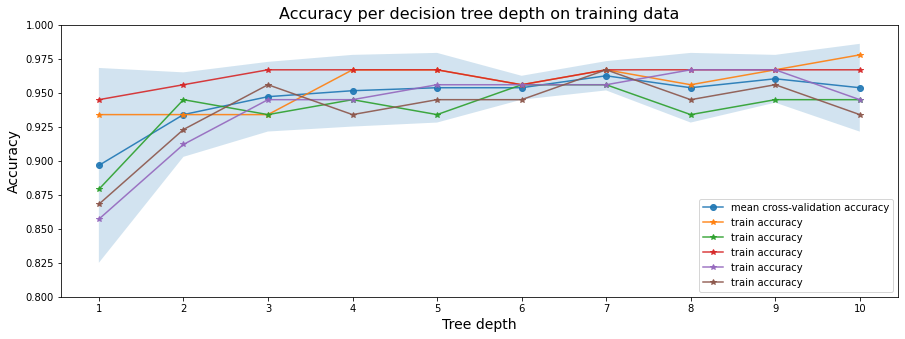
\includegraphics[scale=0.5]{img/acc_depths.png}
        \end{figure}

	The depth with the highest cross-validation average accuracy was 7, which had an accuracy of 0.9649 after training on the entire training set at once and then evaluating on the test set.
	
	\item After generating ROC curves for each feature, the AUCs were collected for each feature. They are displayed below
	\begin{figure}[H]
		\centering
		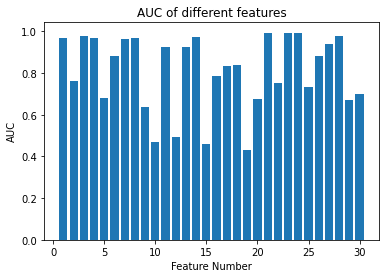
\includegraphics[scale=0.5]{img/aucs.png}
	\end{figure}
	ROC curves were plotted for each picture. Below are seven plots. The first six plots ROC curves for features 1-5, 6-10, 11-15, 16-20, 21-25, and 26-30, respectively. The final plot has the ROC curves for every feature.

	\begin{figure}[H]
		\centering
		\subfloat{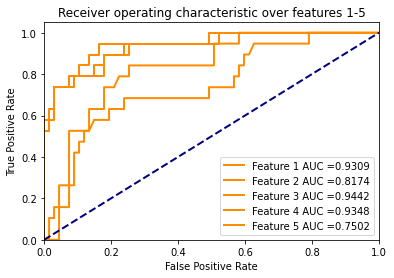
\includegraphics[scale=0.4]{img/roc1.png}}
		\subfloat{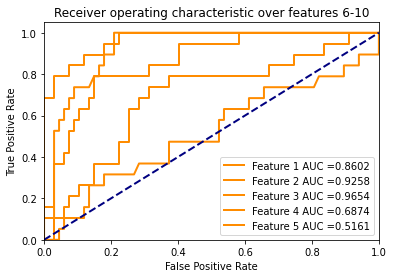
\includegraphics[scale=0.4]{img/roc2.png}}
	\end{figure}
	\begin{figure}[H]
		\centering
		\subfloat{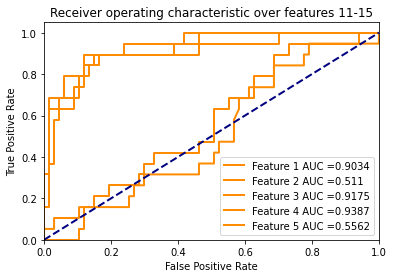
\includegraphics[scale=0.4]{img/roc3.png}}
		\subfloat{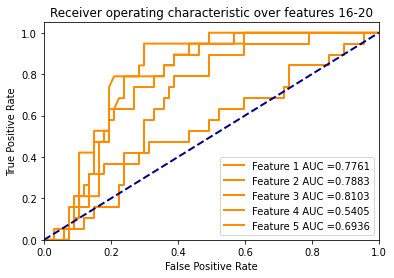
\includegraphics[scale=0.4]{img/roc4.png}}
	\end{figure}
	\begin{figure}[H]
		\centering
		\subfloat{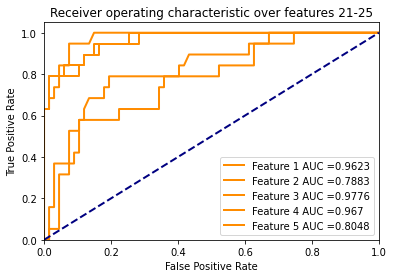
\includegraphics[scale=0.4]{img/roc5.png}}
		\subfloat{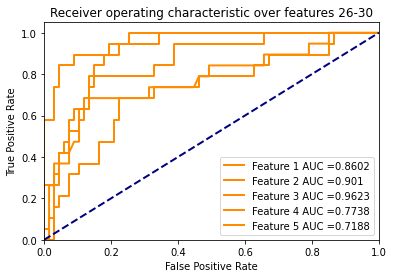
\includegraphics[scale=0.4]{img/roc6.png}}
	\end{figure}
	\begin{figure}[H]
                \centering
                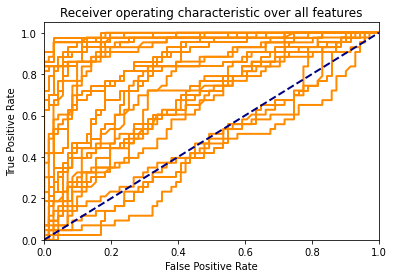
\includegraphics[scale=0.4]{img/roc_all.png}
        \end{figure}

	Based on these ROC curves and the AUC for each feature, some feature seem to be more useful than others for predicting accurate results. Some features, such as features 10, 12, 15, and 19 are little more than random based on their ROC curves and AUC. Other features, such as 1, 3, and 4, have high AUCs and their ROC curves show accurate classification without initially incurring many false positives.

\item The partial AUCs in the range $(0, 0.2)$ for the first five features are plotted (compared to the full AUCs) below.
	\begin{figure}[H]
                \centering
                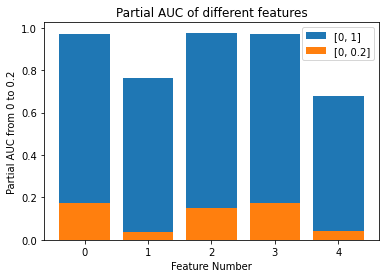
\includegraphics[scale=0.4]{img/partial_auc.png}
        \end{figure}
	The values of each partial AUC are reported in the following table.
	\begin{center}
		\begin{tabular}{|c|c|}
			\hline
			\multicolumn{2}{|c|}{Partial AUC} \\
			\hline
			\textbf{Feature} & \textbf{Value} \\  
			\hline
			1 & 0.1713 \\
			2 & 0.0382 \\
			3 & 0.1490 \\
			4 & 0.1718 \\
			5 & 0.0401 \\
			\hline
		\end{tabular}
	\end{center}

	\item
	The model reliance for each feature, calculated by randomly scmrabling the column corresponding to that feature, is plotted below.
	\begin{figure}[H]
                \centering
                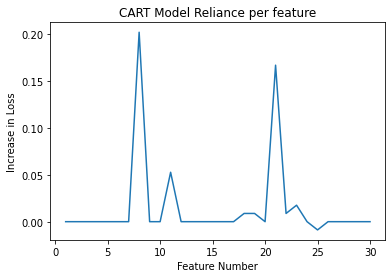
\includegraphics[scale=0.5]{img/model_reliance.png}
        \end{figure}
	The only features which resulted in different accuracies are reported in the following table.
	\begin{center}
		\begin{tabular}{|c|c|}
			\hline
			\multicolumn{2}{|c|}{Model Reliance} \\
			\hline
			\textbf{Feature} & \textbf{Increase in Loss} \\
			\hline
			7 & 0.2018 \\
			10 & 0.0526 \\
			17 & 0.0088 \\
			18 & 0.0088 \\
			20 & 0.1667 \\
			21 & 0.0088 \\
			22 & 0.0175 \\
			24 & -0.0088 \\
			\hline
		\end{tabular}
	\end{center}
	
\end{enumerate}

\item
\begin{enumerate}
	\item
	In the training set there are 290 class 0 examples and 52 class 1 examples, a ratio of 5.57 of class 0 for every class 1. In the test set there are 67 class 0 and 19 class 1, a ratio of 3.53. Overall, there are 357 class 0 and 71 class 1, a ratio of 5.03.

	\item
	For the base algorithms, the final confusion matrices are as follows.
	\begin{center}
		\begin{tabular}{|c|c|c|}
			\hline
			\multicolumn{3}{|c|}{Random Forest} \\
			\hline
			& $\hat{y}=0$ & $\hat{y}=1$ \\
			\hline
			$y=0$ & 66 & 1 \\
			$y=1$ & 1 & 18 \\
			\hline
		\end{tabular}
                \begin{tabular}{|c|c|c|}
                        \hline
                        \multicolumn{3}{|c|}{CART} \\
                        \hline
                        & $\hat{y}=0$ & $\hat{y}=1$ \\
                        \hline
                        $y=0$ & 65 & 2 \\
                        $y=1$ & 3 & 16 \\
                        \hline
                \end{tabular}
                \begin{tabular}{|c|c|c|}
                        \hline
                        \multicolumn{3}{|c|}{ID3} \\
                        \hline
                        & $\hat{y}=0$ & $\hat{y}=1$ \\
                        \hline
                        $y=0$ & 65 & 2 \\
                        $y=1$ & 3 & 16 \\
                        \hline
                \end{tabular}
        \end{center}

	\item
	After setting the max dept for each method to 3 to avoid overfitting, we increasing the weight for class 1 points through the range $1, 2, \dots, 20$. The training and test accuracies per class for each method are plotted below.
	\begin{figure}[H]
                \centering
                \subfloat{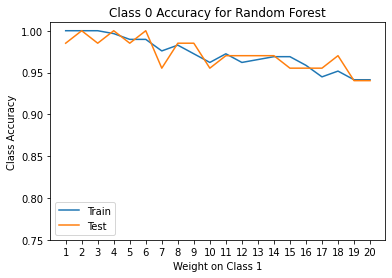
\includegraphics[scale=0.4]{img/forest0.png}}
                \subfloat{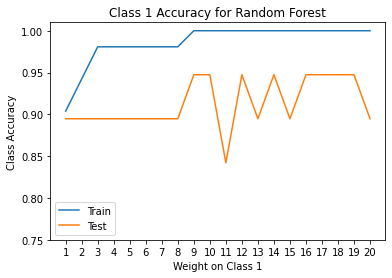
\includegraphics[scale=0.4]{img/forest1.png}}
        \end{figure}
        \begin{figure}[H]
                \centering
                \subfloat{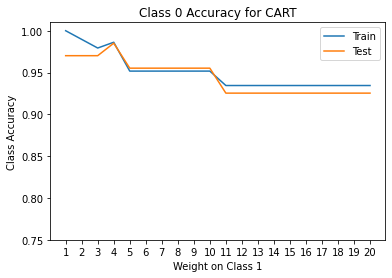
\includegraphics[scale=0.4]{img/cart0.png}}
                \subfloat{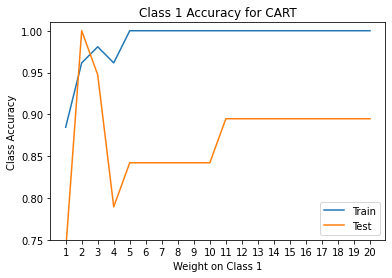
\includegraphics[scale=0.4]{img/cart1.png}}
        \end{figure}
        \begin{figure}[H]
                \centering
                \subfloat{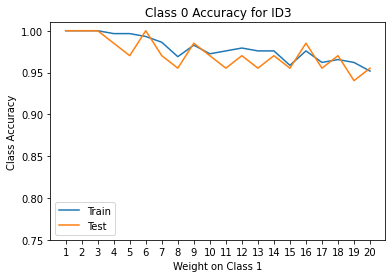
\includegraphics[scale=0.4]{img/id0.png}}
                \subfloat{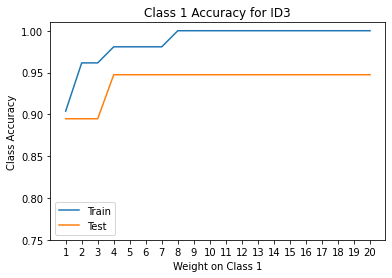
\includegraphics[scale=0.4]{img/id1.png}}
        \end{figure}
	The general trend of these plots is that as the weight of class 1 increases, the accuracy for class 0 decreases and the accuracy for class 1 increases. Another interesting aspect of these plots is that the test accuracy for class 1 does not closely follow the training accuracy, although the test accuracy of class 0 \textit{does} closely follow the training accuracy. This is likely because the small number of class 1 samples makes it harder for the model to generalize to unseen examples.
\end{enumerate}
\end{enumerate}


\end{document}
